\section{Ziel}
\label{sec:Ziel}
Im folgenden Versuch gilt es, die Zeitkonstante eines RC-Gliedes zu bestimmen. Außerdem sollen die Amplitude der Kondensatorspannung sowie die Phasenverschiebung zwischen Generator- und Kondensatorspannung in Abhängigkeit von der Frequenz bestimmt werden. Weiterhin soll gezeigt werden, dass ein RC-Kreis Spannungen integrieren kann.

\section{Theorie}
\label{sec:Theorie}
\subsection{Allgemeine Relaxationsgleichung}
Kehrt ein System nicht oszillatorisch in seinen Ausgangszustand, aus welchem es zuvor entfernt wurde, zurück, wird dies durch Relaxationsvorgänge beschrieben. Die zu betrachtende Größe $A$ besitzt eine Änderungsgeschwindigkeit, welche proportional zu der Abweichung von $A$ zu ihrem asymptotisch erreichbaren Endzustand $A(\infty)$ ist.
\begin{equation}
\label{eqn:dgl}
  \frac{\mathrm{d}A}{\mathrm{d}t} = c[A(t)-A(\infty)]
\end{equation}

Integriert man diese Gleichung vom Zeitpunkt 0 bis zu einem Zeitpunkt t, folgt
\begin{equation}
  A(t) = A(\infty) + [A(0) - A(\infty)]e^{ct}
\end{equation}
mit $c > 0$, da A beschränkt sein muss.

\begin{figure}
  \centering
  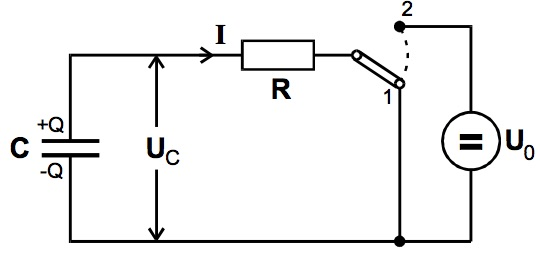
\includegraphics[scale=0.5]{content/RC-Kreis.jpg}
  \caption{Schaltung eines RC-Kreises, Entladung (Stellung 1) und Aufladung (Stellung 2). \cite{anleitung353}.}
  \label{fig:rc-kreis}
\end{figure}

Zunächst wird der Entladevorgang betrachtet. Auf dem Kondensator mit der Kapazität $C$ befindet sich die Ladung $Q$. Für die Spannung zwischen den Kondensatorplatten gilt
\begin{equation}
  U_{\mathrm C} = \frac{Q}{C} .
\end{equation}
Außerdem gilt das ohmsche Gesetz
\begin{equation}
  U = R \cdot I
\end{equation}
sowie $\mathrm{d}Q = I \mathrm{d}t$.  Damit ergibt sich eine eine Differentialgleichung analog zu \ref{eqn:dgl} mit der Randbedingung $Q(\infty)  = 0$, dessen Lösung

\begin{equation}
  Q(t) = Q(0) e^{\frac{-t}{RC}}
\end{equation}
ist, mit $RC$ als Zeitkonstante.

Für die Spannung gilt dementsprechend
\begin{equation}
  \label{a}
  U(t) = U(0) e^{\frac{-t}{RC}}
\end{equation}

Ananlog ergibt sich für den Aufladevorgang mit den Randbedingungen $Q(0) = 0$ und $Q(\infty) = CU_0$
\begin{equation}
  Q(t) = CU_0(1 - e^{\frac{-t}{RC}})
\end{equation}
mit $U_0$ als Spannung der anliegenden Spannungsquelle.

\subsection{Relaxationsphänomene unter Einfluss periodischer Auslenkungen}

\begin{figure}
  \centering
  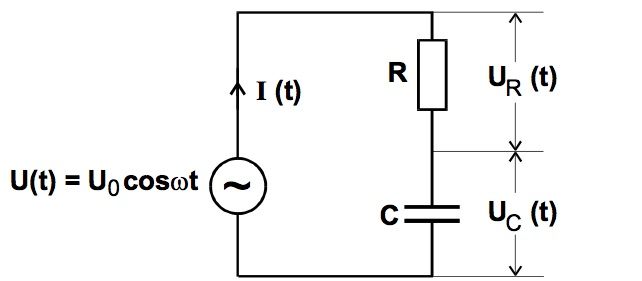
\includegraphics[scale=0.5]{content/RC-periodisch.jpg}
  \caption{Schaltung eines RC-Kreises mit Wechselspannung betrieben, sodass periodische Auslenkungen auftreten.\cite{anleitung353}.}
  \label{fig:rc-periodisch}
\end{figure}

Die nun anliegende Spannung ist eine Sinusspannung. Gilt für die Kreisfrequenz der anliegenden Spannung $\omega \ll \frac{1}{RC}$, ist die Spannung am Kondensator $U_C(t)$ gleich der anliegenden Spannung $U(t)$.
Steigt die Anregungsfrequenz, entsteht eine Phasenverschiebung $\phi$ zwischen den beiden Spannungen mit vorauseilender Generatorspannung. Außerdem nimmt die Amplitude der Kondensatorspannung mit zunehmender Frequenz ab. Für die Spannung am Kondensator gilt allgemein

\begin{equation}
  U_C(t) = A(\omega) \cos (\omega t + \phi(\omega))
\end{equation}

Mit Hilfe der Kirchhoffschen Gesetze
\begin{enumerate}
  \item In einem Knotenpunkt ist die Summe aller Ströme gleich Null.
  \begin{equation}
    \mathrm\sum_{k} I_k = 0
  \end{equation}
  \item In einer abgeschlossenen Masche ist die Summe aller Spannungen gleich Null.
  \begin{equation}
    \mathrm\sum_{k} U_k = 0
  \end{equation}
\end{enumerate}

ergibt sich für die Phasenverschiebung

\begin{equation}
  \label{eqn:phase}
  \phi(\omega) = \arctan(-\omega RC).
\end{equation}

Die Formel zeigt, dass die Phasenverschiebung für kleine Frequenzen gegen 0 und für große Frequenzen gegen $\frac{\pi}{2}$ geht.

Für die frequenzabhängige Amplitude gilt
\begin{equation}
  \label{eqn:amplitude}
  A(\omega) = \frac{U_0}{\sqrt{1 + \omega^2R^2C^2}}.
\end{equation}

Hier ist erkennbar, dass sich $A(\omega)$ bei kleinen Frequenzen $U_0$ nähert und sich bei großen Frequenzen 0 nähert. Da RC-Glieder nur kleine Frequenzen passieren lassen, werden diese als Tiefpässe verwendet.

\subsection{Der RC-Kreis als Integrator}
Unter bestimmten Bedingungen kann ein RC-Glied als Integrator eingesetzt werden. Dazu muss $\omega \gg \frac{1}{RC}$ erfüllt sein. Nach der Kirchhoffschen Maschenregel gilt:
\begin{equation}
  U(t) = U_\mathrm{R}(t) + U_\mathrm{C}(t) = I(t) \cdot R + U_\mathrm{C}(t)
\end{equation}

Mit $I(t) = \frac{\mathrm{d}Q}{\mathrm{d}t} = C \frac{\mathrm{d}U_\mathrm{C}}{\mathrm{d}t}$ und $\omega \gg \frac{1}{RC}$ gilt:

\begin{equation}
  U_C(t) \approx \frac{1}{RC} \int_0^t U(t') \mathrm{d}t'
\end{equation}

da $\left|U_{\mathrm C}\right| \ll \left|U_{\mathrm R}\right|$ und $\left|U_{\mathrm C}\right| \ll \left|U\right|$, wenn $\omega \gg \frac{1}{RC}$.
